\documentclass{beamer}

%\setbeameroption{show notes}

% Vary the color applet  (try out your own if you like)
%\colorlet{structure}{red!65!black}

%\beamertemplateshadingbackground{yellow!100}{white}

%\usepackage{beamerthemesplit}
\usepackage{tikz}
\usepackage{graphics}
\usepackage{graphicx}
\usepackage{hyperref}
\usepackage{setspace}
\usepackage{colortbl}
\usepackage{listings}
\usepackage{amsfonts}
\usepackage{amsmath}
\usepackage{multicol}

%\usetikzlibrary{shapes}

\newcounter{exercise}
\setcounter{exercise}{0}

\newenvironment{exercise}[1]
  {\stepcounter{exercise}\begin{block}{\bf Exercise \arabic{exercise}: #1}}
  {\end{block}}

\lstset{ %
language=Python,                % choose the language of the code
basicstyle=\footnotesize \tt,       % the size of the fonts that are used for the code
%numbers=left,                   % where to put the line-numbers
%numberstyle=\footnotesize,      % the size of the fonts that are used for the line-numbers
%stepnumber=2,                   % the step between two line-numbers. If it's 1 each line will be numbered
%numbersep=5pt,                  % how far the line-numbers are from the code
%backgroundcolor=\color{white},  % choose the background color. You must add \usepackage{color}
%showspaces=false,               % show spaces adding particular underscores
%showstringspaces=false,         % underline spaces within strings
%showtabs=false,                 % show tabs within strings adding particular underscores
%frame=single,                   % adds a frame around the code
%tabsize=2,                      % sets default tabsize to 2 spaces
%captionpos=b,                   % sets the caption-position to bottom
%breaklines=true,                % sets automatic line breaking
%breakatwhitespace=false,        % sets if automatic breaks should only happen at whitespace
%escapeinside={\%*}{*)}          % if you want to add a comment within your code
}

\usetheme{Madrid} 
\useinnertheme{rounded}
\usecolortheme{crane}

\definecolor{dredcolor}{rgb}{.5,0.0,0.0}
\definecolor{blackcolor}{rgb}{0.0,0.0,0.0}
\definecolor{dgreencolor}{rgb}{0.0,0.4,0.0}
\definecolor{dbluecolor}{rgb}{.02,.02,.808}
\newcommand{\dblue}{\color{dbluecolor}\bf}
\newcommand{\dgreen}{\color{dgreencolor}\bf}


\title[Cython]{Cython}
\author[Seljebotn]{Dag Sverre Seljebotn \\ \texttt{d.s.seljebotn@astro.uio.no}}
\date[Oslo Python, June 18, 2013]{Oslo Python Meetup, June 18, 2013}
\institute[ITA, Uni. of Oslo]{Institute of Theoretical Astrophysics, University of Oslo}

%\pgfdeclaremask{fsu}{fsu_logo_ybkgrd}
%\pgfdeclareimage[mask=fsu,width=1cm]{fsu-logo}{fsu_logo_ybkgrd}

%\logo{\vbox{\vskip0.1cm\hbox{\pgfuseimage{fsu-logo}}}}

\begin{document}

  \frame
  {
    \titlepage
    \begin{center}
    \includegraphics[scale=0.4]{cython-logo.png}
    \end{center}
  }


\begin{frame}
\frametitle{What is Cython?}

\begin{itemize} 
\item<+-> Hybrid of Python and C/C++
  \begin{itemize}
  \item {\em Almost} a superset of Python
  \item Can do almost everything you can in C
  \end{itemize}
\item<+-> Integrated with the CPython runtime
   \begin{itemize}
   \item {\tt import mycythoncode}
   \end{itemize}
\end{itemize}

\end{frame}

%\frame{
%  \begin{center}
%    (Demo)
%  \end{center}
%}

\frame{
  \frametitle{Why?}

\uncover<+->{
  \begin{center}
    {\bf Bridge Python and C}
  \end{center}
}
~

\begin{itemize}
\item<+-> pyzmq, lxml, pymssql, hdf4py, pytables, mpi4py, ...
\item<+-> Translating idiomatic C/C++ to idiomatic Python
  \begin{itemize}
  \item (vs. SWIG, ctypes, cffi)
  \end{itemize}
\end{itemize}

}


\frame{
  \frametitle{Why?}

\uncover<+->{
  \begin{center}
    {\bf Speed!}
  \end{center}


  \begin{columns}[t]
    \begin{column}{0.3\textwidth}
      Python \\ High-level \\ Slow \\ No variables typed
    \end{column}
    \begin{column}{0.4\textwidth}
      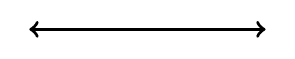
\begin{tikzpicture}
	\draw[<->, very thick]  (0, 0)  -- (3, 0);
      \end{tikzpicture}
    \end{column}
    \begin{column}{0.3\textwidth}
      C/C++/Fortran \\ Lower-level \\ Fast \\ All variables typed
    \end{column}
  \end{columns}
}  

~

  \begin{itemize}
  \item<+-> For CPU-intensive workloads, Python is slow
    \begin{itemize}
    \item As in 100x to 1000x slower
    \end{itemize}
    \item<+-> Cython: Incremental optimization workflow
      \begin{itemize}
      \item Optimize, don't re-write
    \end{itemize}

  \item<+-> De facto standard for writing scientific Python libraries
    \begin{itemize}
    \item Pandas, scikits-learn, parts of SciPy, Sage, tons of domain-specific
    \item Often combines number crunching and calling C/Fortran code
    \end{itemize}

  \end{itemize}


}

\frame{
  \frametitle{Not a usecase: Static type checking}
  \begin{itemize}
    \item<+-> Cython is (partially) statically typed because it has too,
      not because it wants to
    \item<+-> You still need to run the program to catch a typo
  \end{itemize}
}


%\frame{
%  \frametitle{Some words of caution...}
%  \begin{itemize}
%  \item<+-> Development of Cython primarily driven by need
%    \begin{itemize}
%    \item Pragmatic or ugly?
%    \end{itemize}
%  \item<+-> Great mailing list support...
%  \item<+-> ...but documentation can be lacking
%  \end{itemize}
%}

\frame{
  \frametitle{How does it work?}

  \begin{enumerate}
  \item<+-> Write Cython source code ({\tt hello.pyx})
  \item<+-> Use {\tt cython} to convert to C using the CPython API
    ({\tt hello.c})
  \item<+-> Build using C compiler ({\tt hello.c}) to produce shared
    library ({\tt hello.so} or {\tt hello.pyd})
  \item<+-> {\tt import hello}
  \end{enumerate}
}


\frame{
  \frametitle{Ways to build Cython code...}

  \begin{itemize}
  \item<+-> \texttt{distutils}: \texttt{setup.py} and \texttt{cythonize()}
  \item<+-> IPython notebook
  \item<+-> Simple cases: \texttt{pyximport} automatically compiles on Python import
  \item<+-> Advanced cases: Use a {\em real} build tool
    \begin{itemize}
    \item CMake, waf, SCons, Unix Makefiles, IDE projects...
    \end{itemize}
  \end{itemize}

}


\frame{
  \begin{center}
    (demo on ways to build)
  \end{center}
}

\frame{
  \begin{center}
    (demo on speeding up image blur)
  \end{center}
}

\frame{
  \begin{center}
    (demo on calling libpng)
  \end{center}
}


\frame{
  \frametitle{Using Cython as a language on its own}
In addition to Python and C, Cython has its own features:
  \begin{itemize}
    \item<+-> Compile-time inclusion of other Cython code using {\tt pxd}-files
      and {\tt cimport}
    \item<+-> Avoid overhead of Python function calls with {\tt cdef}-functions
    \item<+-> Avoid overhead of Python classes with {\tt cdef}-classes
  \end{itemize}
}

\frame[containsverbatim]{
  \frametitle{Cython syntax: cdef functions}
  Calling a {\tt def} function a) has a large performance penalty,
  can only accept Python-compatible arguments (no pointers).


~

Syntax for declaring a Cython-only function:
\lstset{emph={cdef, cpdef, double},emphstyle=\color{blue}} 
\begin{lstlisting}
cdef double f(double x) except *:
    return x**3 + 2*x**2
\end{lstlisting}

~

Not available from Python-space. Use {\tt cpdef} to make a fast version
available to Cython and a slower one to Python:
\begin{lstlisting}
cpdef double f(double x) except *:
    return x**3 + 2*x**2
\end{lstlisting}

}


\frame[containsverbatim]{
  \frametitle{Classes}
  Cython has two kinds of classes:
  \begin{itemize}
    \item {\tt class MyClass}: Exactly like in Python
    \item {\tt cdef class MyClass}:
      \begin{itemize}
	\item Store typed attributes (avoid converting to/from Python object)
	\item Faster method calls when called from Cython and declaration known
          compile-time
      \end{itemize}
  \end{itemize}
\begin{lstlisting}
cdef class MyClass:
    cdef int value
    cpdef int some_method(self, int arg):
        ...
\end{lstlisting}

~

Normal Python classes can inherit from cdef classes, but not the other
way around.  }

\frame[containsverbatim]{
  \frametitle{cdef class polymorphism}
  Methods of cdef class objects can be called much faster than methods 
  on regular objects, {\em if} the variable is typed.

~

\begin{lstlisting}
untyped = MyClass(arg1, arg2)
cdef MyClass typed = untyped
untyped.some_cpdef_method() # slow
typed.some_cpdef_method() # fast
\end{lstlisting}
  
~
  Regular Python classes can not be used as the type of
  a variable.
}

\frame[containsverbatim]{
  \frametitle{cdef class attributes}
  Attributes are different from regular classes:
  \begin{itemize}
    \item All attributes must be pre-declared at compile-time
    \item Declare accessability
  \end{itemize}

~

\begin{lstlisting}
cdef class SineWave(DoubleFunction):
    cdef double offset # not available in Python-space
    cdef public double frequency # available in Python-space
    property period:
        def __get__(self): return 1.0 / self.frequency
	def __set__(self, value): self.frequency = 1.0 / value
    ...
\end{lstlisting}

}

\frame{
  \frametitle{cdef class caveats}
  Special methods have some differences from regular classes:
  \begin{itemize}
    \item<+-> {\tt \_\_cinit\_\_} and {\tt \_\_dealloc\_\_} for allocating/freeing
      C data structures belonging to the object
    \item<+-> Arithmetic operators, pickling etc. are different
  \end{itemize}
}

\frame[containsverbatim]{
  \frametitle{The None issue}
  \begin{itemize}
    \item For convenience, variables declared as having a cdef class type can
      be assigned {\tt None}.
    \item By default, accessing None in such a ``typed'' fashion will
      lead to undefined behaviour (hopefully a crash). Always test with {\tt is None}
      first!
    \item The {\tt nonecheck} {\em compiler directive} will raise an exception instead;
      but slows down all such accesses.
  \end{itemize}

\begin{lstlisting}
import cython
@cython.nonecheck(True)
def func():
    cdef MyClass obj = None
    try:
        print obj.myfunc() # raises exception
    except AttributeError:
        pass
    with cython.nonecheck(False):
        print obj.myfunc() # hope for a crash!
\end{lstlisting}

}


\frame{
  \frametitle{Opinions}
\begin{itemize}
\item<+-> Cython is not elegant but it does many jobs well.
\item<+-> Cython is a supplement. {\bf Do not} use Cython as
  your main programming language.
\item<+-> For speed: Look at Numba (scientific/number crunching) or
  PyPy (other domains) after making sure they will work for you.
\end{itemize}


}


\end{document}
